\documentclass[11pt,a4paper,oneside]{report}
\usepackage[T1]{fontenc}
\usepackage[utf8]{inputenc}
\usepackage[italian]{babel}
\usepackage{lmodern,amsmath,amssymb,booktabs,tabularx,longtable,graphicx}
\usepackage[margin=21mm,headheight=15pt]{geometry}
\usepackage{microtype,caption,float,titlesec,fancyhdr}
\usepackage[hidelinks]{hyperref}
\usepackage{url}
\hypersetup{pdftitle={Music Discovery: Contextual Multi-Armed Bandit},pdfsubject={Relazione di progetto di Sistemi Intelligenti per Internet},pdfkeywords={Music discovery, LinUCB, Last.fm, valutazione offline}}
\graphicspath{{figures/}}
\setlength{\parindent}{1em}
\setlength{\parskip}{2pt}
\linespread{1.0}
\setcounter{tocdepth}{1}
\raggedbottom
\titleformat{\chapter}[hang]{\normalfont\LARGE\bfseries}{\thechapter.}{.6em}{}
\titlespacing*{\chapter}{0pt}{0pt}{14pt}
\titlespacing*{\section}{0pt}{10pt}{4pt}
\AtBeginDocument{%
 \setlength{\abovedisplayskip}{7pt plus 2pt minus 2pt}%
 \setlength{\belowdisplayskip}{7pt plus 2pt minus 2pt}%
 \setlength{\abovedisplayshortskip}{4pt plus 2pt}%
 \setlength{\belowdisplayshortskip}{5pt plus 2pt minus 2pt}}
\captionsetup{font=small,labelfont=bf}
\pagestyle{fancy}
\fancyhf{}\fancyhead[L]{\small Music Discovery CMAB}\fancyhead[R]{\small Relazione di progetto}
\fancyfoot[C]{\thepage}
\renewcommand{\headrulewidth}{.3pt}
\newcommand{\autore}{Michele Arietta}
\newcommand{\matricola}{637929}
\newcommand{\corsostudi}{Laurea magistrale in Ingegneria Informatica\\[.15cm](curriculum Intelligenza Artificiale e Machine Learning)}
\newcommand{\docente}{Giuseppe Sansonetti}
\newcommand{\annoaccademico}{2025/2026}
\newcommand{\metric}[1]{\texttt{\detokenize{#1}}}
\newcommand{\figura}[4]{\begin{figure}[htbp]\centering\includegraphics[width=#2\linewidth]{#1}\caption{#3}\label{#4}\end{figure}}
\begin{document}
\hypersetup{pageanchor=false}
\begin{titlepage}
\centering
{\Large Università degli Studi Roma Tre\par}
\vspace{.5cm}
{\large \corsostudi\par}
\vspace{1.8cm}
{\Huge\bfseries Music Discovery\par}
\vspace{.35cm}
{\LARGE Contextual Multi-Armed Bandit per la scoperta musicale\par}
\vspace{.8cm}
{\large Progettazione, simulazione sequenziale offline\\e valutazione su Last.fm 1K\par}
\vfill
{\large Progetto per l'esame di Sistemi Intelligenti per Internet\par}
\vspace{.8cm}
\begin{tabular}{ll}
Studente & \autore\\
Matricola & \matricola\\
Docente & \docente\\
Anno accademico & \annoaccademico
\end{tabular}
\vfill
{\small Relazione basata sulle esecuzioni ufficiali di validation e test held-out.\\
Parametri selezionati sulla validation e congelati prima del test.}
\end{titlepage}
\hypersetup{pageanchor=true}
\pagenumbering{roman}
\chapter*{Abstract}
La raccomandazione musicale deve conciliare la continuità con gli interessi dell'utente e la proposta di contenuti non ancora ascoltati. Questo progetto studia tale compromesso attraverso un Contextual Multi-Armed Bandit, implementato come simulazione sequenziale offline sugli eventi di Last.fm 1K. Il sistema tratta un item come coppia coerente di identità della traccia e dell'artista, costruisce candidati esclusivamente dal passato osservabile e impiega un contesto di quindici componenti: tredici variabili numeriche standardizzate e due indicatori binari di novelty.

Il protocollo comprende un warm-up storico, una validation cronologica e un test held-out. La reward è il logaritmo di uno più il numero di ascolti futuri dell'artista nella finestra di sette giorni; diventa disponibile all'apprendimento soltanto alla fine di tale finestra. Sono confrontati Random, Global Popularity, Personalized Greedy, $\varepsilon$-Greedy e LinUCB. Le 36 configurazioni di validation includono tre profondità dei pool; la selezione è svolta esclusivamente nello scenario principale $N=100$, fissato prima dei risultati. Vengono così congelati $\alpha=2$ per LinUCB ed $\varepsilon=0{,}05$ per $\varepsilon$-Greedy.

Nel test, su 562 utenti e 82.905 decision point, Personalized Greedy ottiene NDCG@10 pari a 0,258795 e LinUCB 0,257741. Un bootstrap appaiato per utente con 10.000 replicazioni produce per la loro differenza un intervallo di confidenza al 95\% pari a $[-0{,}006601;\,0{,}004389]$. LinUCB mostra invece incrementi di track novelty, artist novelty e diversità, accompagnati da una riduzione della reward media. Il risultato supporta un compromesso descrittivo fra accuratezza e scoperta, senza stabilire una superiorità assoluta di LinUCB o un effetto causale sulle abitudini musicali.

La relazione documenta il collegamento fra codice, scelte sperimentali e artefatti verificati. Non si tratta di una valutazione controfattuale IPS/SNIPS: Last.fm registra ascolti, ma non esposizioni a raccomandazioni, propensioni di logging o risposte causate dal sistema.
{\small\tableofcontents}
\clearpage\pagenumbering{arabic}
\chapter{Problema, obiettivi e contributi}\label{ch:intro}
Un utente può apprezzare una raccomandazione perché conferma un gusto consolidato oppure perché introduce un artista nuovo. Le due finalità non coincidono: massimizzare la probabilità di ritrovare contenuti già ascoltati può concentrare l'esposizione su una parte ridotta del catalogo; introdurre contenuti molto diversi può aumentare la varietà ma ridurre la pertinenza immediata. Nel dominio musicale, inoltre, il riascolto è un comportamento naturale. L'assenza di novità non costituisce da sola un errore, così come la presenza di un artista mai ascoltato non garantisce un'esperienza positiva.

Il rischio di una \emph{filter bubble} motiva lo studio dell'esplorazione, ma richiede osservazioni sul comportamento e sull'esposizione per essere misurato direttamente. Questo lavoro impiega una definizione più circoscritta di scoperta: una traccia o un artista sono nuovi se non compaiono nella storia disponibile prima della decisione. La novelty così definita è verificabile nei log e distingue l'ampiezza delle proposte dalla capacità di anticipare gli ascolti futuri.

La domanda di ricerca è la seguente: \emph{un modello contestuale con esplorazione può mantenere un'accuratezza di ranking vicina a quella di una baseline personalizzata, aumentando al contempo novelty e diversità delle liste?} Per rispondere occorrono sia un riferimento che sfrutti gli interessi storici, sia strategie che se ne discostino casualmente o in funzione del contesto. La valutazione deve quindi osservare insieme pertinenza e composizione delle proposte, anziché identificare la scoperta con il solo reward. Le policy condividono lo spazio di azioni, ma possono usare segnali diversi.

\section{Scelte progettuali}
Il CMAB consente di rappresentare decisioni ripetute su un catalogo osservabile che cambia, usando storia dell'utente e proprietà dei candidati per orientare l'esplorazione. Il feedback differito è necessario perché il proxy scelto accumula ascolti su più giorni: anticiparlo renderebbe disponibili informazioni non ancora maturate. A ogni inizio di sessione si produce un ranking e si sceglie una sola azione Top-1; la Top-K serve alla valutazione, non rappresenta K azioni premiate.

Il progetto privilegia la tracciabilità della simulazione. Le identità sono condivise fra i moduli; lo stato incrementale esclude gli eventi al timestamp corrente; le statistiche di scala derivano soltanto dai contesti di warm-up. La distinzione fra raccomandazione track-level e rilevanza artist-level è esplicita: le Top-K tracce vengono convertite in una sequenza di artisti distinti per Precision, Recall e NDCG. Questa scelta evita che ripetere lo stesso artista generi più rilevanze indipendenti.

\section{Contributo e perimetro delle conclusioni}
I contributi sono un simulatore causale con feedback differito, un confronto riproducibile fra cinque famiglie di policy, una selezione congelata prima del test e un'analisi dell'incertezza che mantiene raggruppate le decisioni dello stesso utente. I risultati includono anche esempi musicali autentici, utili per interpretare le liste al di là delle medie.

In un sistema online l'esplorazione potrebbe cambiare le esposizioni e raccogliere nuove risposte. Qui la sequenza Last.fm rimane fissa: raccomandare un artista non ne modifica gli ascolti futuri. Si studia quindi la traiettoria decisionale del bandit rispetto a un proxy osservato, non la sua capacità causale di cambiare i gusti. Questa distinzione motiva la lettura congiunta delle metriche del Capitolo~\ref{ch:metodo} e delimita le conclusioni.

\chapter{Fondamenti e algoritmi}\label{ch:teoria}
\section{Dal recommender al bandit contestuale}
Nel Multi-Armed Bandit classico una policy sceglie un'azione $a_t$ e riceve la sola ricompensa associata alla scelta. L'esplorazione acquisisce informazione su alternative incerte; l'exploitation sfrutta le stime correnti. UCB aggiunge alla media empirica un bonus di incertezza:
\begin{equation}
 U_a(t)=\widehat{\mu}_a(t)+\sqrt{\frac{2\ln t}{n_a(t)}},
\end{equation}
per azioni con $n_a(t)>0$, nel caso classico di reward indipendenti, stazionari e limitati in $[0,1]$ per ciascun braccio \cite{auer2002}. UCB1 inizializza provando ogni azione almeno una volta; equivalentemente, un'azione non osservata ha priorità esplorativa. La formula fornisce soltanto l'intuizione: il progetto implementa LinUCB, non UCB1.

Nel CMAB il vettore $x_{u,a,t}\in\mathbb{R}^{d}$ riassume utente, item e stato prima della decisione. Generalizzare fra candidati è utile quando non tutti gli item hanno feedback individuali sufficienti. Qui $d=15$ e $\mathcal A_u(t)$ varia; il ritardo separa decisioni e aggiornamenti disponibili.

\section{LinUCB effettivamente implementato}
Il modello lineare condiviso usa una matrice $A\in\mathbb{R}^{15\times15}$ e un vettore $b\in\mathbb{R}^{15}$, inizializzati con $A=I$ e $b=0$. Non sono mantenute matrici separate per ciascuna traccia o ciascun utente. Date le sole azioni con feedback maturo, valgono
\begin{align}
A_t &= I+\sum_{\tau:\,\tau+\Delta\leq t}x_\tau x_\tau^\top,
&b_t &= \sum_{\tau:\,\tau+\Delta\leq t}r_\tau x_\tau,\\
\widehat{\theta}_t&=A_t^{-1}b_t,
&s(x)&=x^\top\widehat{\theta}_t+
\alpha\sqrt{x^\top A_t^{-1}x}.\label{eq:linucb}
\end{align}
Il vettore $x_\tau$ è quello standardizzato al momento della decisione, conservato nel feedback. Il parametro $\alpha$ controlla il bonus; $\alpha=0$ conserva soltanto la stima lineare, senza diventare la baseline Personalized Greedy. La regola deriva dall'approccio LinUCB \cite{li2010}, adattato qui a un modello condiviso sulle feature delle azioni.

Il codice usa Cholesky e sostituzioni triangolari senza costruire l'inversa. La selezione non modifica $A,b$; solo il feedback maturo della Top-1 applica $A\leftarrow A+xx^\top$, $b\leftarrow b+rx$. Non esiste un'intercetta esplicita: manca un livello di base liberamente stimabile e, per $x=0$, la componente media è zero. La personalizzazione passa dal contesto, con coefficienti condivisi. Il reward logaritmico non è limitato a $[0,1]$: non si rivendicano garanzie di regret derivate per altre distribuzioni.

\section{Baseline e interpretazione del confronto}
Random, permutazione uniforme con generatore isolato, rappresenta l'esplorazione non personalizzata. Global Popularity usa gli ascolti globali dell'artista come riferimento aggregato. Personalized Greedy sfrutta invece le preferenze storiche mediante il conteggio utente--artista, con tie-break per popolarità della traccia e chiave canonica. Il confronto distingue così il valore della personalizzazione da quello dei segnali globali, entro lo stesso pool.

$\varepsilon$-Greedy introduce una dose controllata di esplorazione casuale: con probabilità $\varepsilon$ permuta il pool, altrimenti usa l'intero ranking Greedy. Il ramo è estratto una volta per decisione e riguarda anche la Top-K. Non apprende medie di reward. LinUCB guida invece le scelte con stima contestuale e incertezza, studiando un'alternativa al distacco casuale dalle preferenze storiche.

Le strategie coprono diversi compromessi exploration--exploitation, ma LinUCB cambia anche rappresentazione e apprendimento: senza ablation il confronto non isola causalmente il solo bonus UCB.

\chapter{Dataset, analisi esplorativa e preprocessing}\label{ch:dati}
\section{Struttura e attività degli utenti}
Last.fm 1K raccoglie eventi acquisiti attraverso \emph{user.getRecentTracks}; il README locale dichiara una riga per ascolto e sei campi separati da tab: utente, timestamp, artist MBID, nome artista, track MBID e titolo \cite{lastfm}. Il file completo contiene 19.150.868 righe e 992 utenti. Il profilo anagrafico separato non entra nelle feature del modello. Gli eventi sono osservazioni implicite di ascolto, non giudizi espliciti né click su raccomandazioni del sistema.

Il notebook \metric{01_dataset_analysis.ipynb} distingue un campione iniziale di 100.000 righe dalla scansione esplorativa completa. Il campione contiene soltanto quattro utenti: le sue percentuali non sono quindi trattate come stime rappresentative dell'intera popolazione. Le statistiche complete mostrano una forte eterogeneità: gli eventi per utente hanno media 19.305,31, mediana 11.551, minimo 2 e massimo 183.103. Il primo e il terzo quartile sono 3.774,25 e 25.707,75. Si sceglie la macro-media per assegnare pari peso agli utenti; una media per decisione attribuirebbe più peso ai profili con più sessioni e rappresenterebbe un diverso obiettivo di aggregazione.

\figura{eda_activity.png}{.91}{Distribuzione degli ascolti per utente: numero di eventi sull'asse orizzontale e utenti in scala logaritmica su quello verticale. Output originale della cella 21 del notebook EDA, ingrandito per leggibilità; nessuna nuova scansione.}{fig:activity}

Le entità esplorative contate nel notebook sono 176.892 artisti e 1.505.209 tracce. Tali numeri dipendono dai criteri di identificazione usati nell'EDA e non rappresentano automaticamente il numero di item canonici della pipeline definitiva. In particolare, l'identità operativa finale include l'artista anche quando esiste un track ID. Analogamente, il catalogo per la coverage è la sola unione dei candidati esposti nella fase: usare il conteggio globale EDA come denominatore cambierebbe la metrica.

\clearpage
\section{Concentrazione, ripetizione e sparsità}
La popolarità è molto concentrata. Nel conteggio esplorativo, l'1\% degli artisti raccoglie il 62,7254\% degli ascolti e il 10\% il 91,9006\%. Per le tracce le quote corrispondenti sono 31,8500\% e 71,1172\%. La mediana della popolarità è di quattro eventi per artista e due per traccia. Questi dati descrivono una lunga coda con molti contenuti poco supportati. Non è disponibile in questa relazione una misura di densità della matrice canonica utente--item; la sparsità è motivata dall'eterogeneità e dalla coda osservate, senza inventare una percentuale di celle vuote.

\figura{eda_concentration.pdf}{.91}{Concentrazione degli ascolti nell'EDA. Curve ridisegnate dai cinque valori tabulati già salvati nelle celle 39--40 del notebook: nessun ricalcolo dal dataset. La curva degli artisti corrisponde alla Figura originale della cella 41.}{fig:concentration}

Anche la ripetizione individuale è marcata: il tasso medio esplorativo di ripetizione è 0,885690 per artista e 0,664859 per traccia; le mediane sono 0,944116 e 0,724130. Il 10\% degli artisti preferiti da ciascun utente concentra mediamente il 62,9290\% dei suoi ascolti. Questa evidenza giustifica una baseline personalizzata forte e la distinzione fra nuova traccia di artista noto e nuovo artista.

\clearpage
\section{Qualità dei dati e identità canoniche}
L'EDA rileva 602.166 eventi senza artist ID (3,144327\%) e 2.168.588 senza track ID (11,323706\%). Scartarli significherebbe rimuovere una frazione sostanziale della storia. Il loader mantiene i campi vuoti e costruisce fallback espliciti. Il nome esatto dell'artista sostituisce il suo ID soltanto quando questo manca; il titolo sostituisce il track ID soltanto se assente. Maiuscole, spazi significativi e Unicode non sono normalizzati arbitrariamente; un valore composto solo da spazi è considerato mancante. Se non è possibile identificare artista o item, viene sollevato un errore.

Il file è TSV, non CSV con quoting: ogni riga fisica possiede cinque tab. Il parser definitivo usa \metric{QUOTE_NONE}, così le virgolette nei titoli restano letterali. Il controllo a sei colonne rimane attivo. Il precedente comportamento CSV poteva fondere più righe, spiegando perché il notebook preliminare \metric{reward_sessions_split.ipynb} riporti 19.098.853 righe e coorti di 561 utenti. Quegli output servono come motivazione esplorativa, non sostituiscono i 19.150.868 eventi e i 562 utenti delle run ufficiali.

Un secondo problema riguarda track ID attribuiti a più artisti. In record di MF DOOM e Viktor Vaughn compare lo stesso ID:
\begin{quote}\small\path{7aebbc02-17ab-4f94-b91d-ff164c89f1f8}.\end{quote}
L'identità finale è uniforme per tutto il dataset: se presente, il track ID è abbinato all'artist key; altrimenti il titolo esatto è abbinato alla stessa artist key. Tag di tipo e lunghezze dei campi rendono la serializzazione non ambigua. La regola non dipende da collisioni scoperte a posteriori o dalla frequenza futura dell'item.

\section{Tempo, sessioni e motivazione delle soglie}
L'EDA mostra storie molto diverse per durata: la mediana è circa 925,63 giorni. Sono presenti anche timestamp isolati nel 2010 e nel 2013; non vengono corretti inventando date, ma i limiti delle fasi impediscono che entrino nelle metriche sperimentali del 2009.

Il notebook preliminare sui gap osserva che, fra pause inferiori a due ore, il 94,89\% ricade entro dieci minuti. Nei riascolti della stessa traccia, la finestra di sette giorni raccoglie circa il 50,98\% dei gap misurati, contro il 29,98\% a un giorno e il 60,54\% a quattordici. Sono indicazioni esplorative ottenute prima della correzione del parser: motivano le soglie adottate, ma non sono stime aggiornate della reward artist-level.

Nel codice definitivo una sessione inizia al primo evento dell'utente oppure quando il gap dall'evento precedente è \emph{strettamente maggiore} di dieci minuti. Il decision point coincide con quell'evento, che resta escluso dallo stato usato dalla policy. Il caso gap esattamente pari a dieci minuti non apre una nuova sessione. Gli split e l'eleggibilità finale sono formalizzati nel Capitolo~\ref{ch:metodo}.

\paragraph{Implicazioni progettuali dell'analisi esplorativa.}
Concentrazione e ripetizione rendono necessario confrontarsi con una baseline personalizzata forte, ma suggeriscono anche di misurare quante proposte escano dalla familiarità storica. L'eterogeneità motiva il pari peso agli utenti, mentre gli ID mancanti richiedono identità utilizzabili senza perdere eventi. La sequenza degli ascolti impone di aggiornare storia e candidati nel tempo. Le analisi preliminari dei gap orientano sessionizzazione e orizzonte, senza dimostrarne l'ottimalità. Queste osservazioni motivano i requisiti dell'architettura seguente; non costituiscono un confronto sperimentale fra architetture alternative.

\chapter{Architettura e implementazione}\label{ch:sistema}
\section{Separazione fra osservazione, azione e valutazione}
L'architettura separa stato osservabile, policy e ambiente offline per rendere verificabile il confine fra informazione storica e valutazione futura. Distinguere generazione dei candidati, contesto e ranking permette di cambiare policy mantenendo lo stesso spazio d'azione e le stesse osservazioni ammissibili; isolare reward e coda differita impedisce che un feedback calcolabile dall'evaluatore diventi subito apprendimento. La modularità serve quindi causalità e confrontabilità, oltre alla manutenzione del codice.

Il loader conserva tutte le righe in una cache SQLite temporanea ordinata cronologicamente. Stato e candidati si aggiornano incrementalmente; indici e spool limitano la RAM occupata dai record. Sono risposte tecniche al volume dei dati, non alternative architetturali confrontate scientificamente.

Il flusso logico è:
\begin{center}
\fbox{\parbox{.91\linewidth}{\centering
TSV e identità canoniche $\longrightarrow$ eventi cronologici\\[4pt]
$D_{<t}\longrightarrow$ TemporalState $\longrightarrow$ CandidateGenerator\\[4pt]
$\longrightarrow$ ContextBuilder $\longrightarrow$ scaler congelato $\longrightarrow$ policy\\[4pt]
$\longrightarrow$ Top-1 e Top-K $\longrightarrow$ log immutabile e metriche\\[4pt]
Solo Top-1 $\longrightarrow$ reward offline $\longrightarrow$ coda a $t+7d$
$\longrightarrow$ aggiornamento della policy}}
\end{center}
L'accesso al futuro appartiene al calcolatore di reward e al valutatore, non al percorso che costruisce stato, candidati o feature. Ogni policy riceve lo stesso ambiente e lo stesso criterio di eleggibilità. Per ciascuna configurazione vengono costruite istanze indipendenti; non sono condivisi stato mutabile, feedback o flussi casuali.

\section{Stato incrementale e causalità}
Lo stato al decision point è
\begin{equation}
O_t=f(D_{<t}),\qquad D_{<t}=\{e:\operatorname{timestamp}(e)<t\}.\label{eq:state}
\end{equation}
TemporalState conserva conteggi per utente, per coppia utente--item e utente--artista, ultimo timestamp individuale, ascolti globali e utenti distinti per item e artista, oltre alla prima osservazione dell'item. Queste strutture supportano novelty, recency e age senza filtrare nuovamente l'intero dataset per ciascuna decisione.

Gli indici del CandidateGenerator ricevono gli eventi tramite listener solo dopo il loro ingresso nello stato. Per ciascun gruppo valutabile di decisioni simultanee, \metric{run_phase()} applica nell'ordine: feedback con scadenza $\leq t$, avanzamento dello stato a $t$, tutte le decisioni del gruppo e infine ammissione degli eventi a $t$. Candidati e contesti condividono dunque $D_{<t}$; nessuna scelta del gruppo genera un feedback immediato.

La memoria di apprendimento ha una convenzione distinta dallo stato delle feature. Se una decisione precedente è presa a $s$ e $s+7d=t$, la sua reward include gli ascolti esattamente a $t$ e può aggiornare $A,b$ prima delle nuove scelte. Per esempio, un ascolto dell'artista selezionato alle 10:00 dell'8 gennaio conta nel feedback della decisione delle 10:00 del 1 gennaio, ma non nei conteggi o nei candidati delle decisioni delle 10:00 dell'8 gennaio. Il simulatore dà priorità ai feedback maturi rispetto alle decisioni simultanee: non usa ascolti successivi a $t$, ma l'intera informazione del learner non è descritta dal solo $D_{<t}$. È la convenzione implementata per l'uguaglianza dei timestamp, non una disponibilità anticipata rispetto alla scadenza.

Per esempio, se la prima sessione contiene eventi alle 10:00, 10:03 e 10:05 e una nuova sessione inizia alle 10:20, la decisione delle 10:20 osserva i tre eventi precedenti. L'evento delle 10:20 rimane invisibile, anche a un secondo utente che decida nello stesso istante. La costruzione di contesti usa esattamente lo stato avanzato a quel timestamp e rifiuta item con prima osservazione non anteriore a $t$.

\section{Tre pool e unione dei candidati}
Personal dà accesso agli interessi già osservati, Popular aggiunge segnali globali e Discovery ammette item mai ascoltati dall'utente. La loro unione evita di vincolare tutte le policy alla sola storia individuale e definisce un ambiente comune: il generatore stabilisce quali azioni siano disponibili, la policy come ordinarle. La scoperta rimane possibile solo entro questo catalogo osservato.

Per ogni utente si costruisce
\begin{equation}
\mathcal A_u(t)=A_N^{\mathrm{personal}}(u,t)\cup
A_N^{\mathrm{popular}}(t)\cup A_N^{\mathrm{discovery}}(u,t).\label{eq:pool}
\end{equation}
$N\in\{50,100,200\}$ è la profondità di \emph{ciascuna} sorgente, non la cardinalità finale. Dopo la deduplicazione, $|\mathcal A_u(t)|\leq3N$; l'overlap può renderla sensibilmente inferiore. Non si impongono quote fra sorgenti nella lista finale.

Il pool Personal prende i primi $N$ item, in ordine crescente di chiave canonica, fra le tracce osservate degli artisti già conosciuti: comprende così item già ascoltati e item non ascoltati di quegli artisti, senza priorità obbligatoria al primo gruppo. Popular prende i primi $N$ per ascolti globali dell'item prima di $t$, con tie-break sulla chiave. Discovery prende i primi $N$ item mai ascoltati dall'utente nello stesso ordine lessicografico e li etichetta \emph{familiar artist} ($C_{u,i}=0,C_{u,g}>0$) o \emph{new artist} ($C_{u,i}=C_{u,g}=0$). L'etichetta non modifica l'estrazione: non bilancia le due categorie né impone loro quote. La regola è deterministica, ma introduce un possibile bias lessicografico; il generatore non campiona uniformemente il catalogo.

Le sorgenti vengono troncate separatamente, quindi unite nell'ordine Personal, Popular, Discovery. Un duplicato conserva tutti i source flag. L'ordinamento dei pool non coincide con quello della policy: in particolare, Popular usa popolarità \emph{track-level}, mentre la baseline Global Popularity usa popolarità \emph{artist-level}. Tale differenza è intenzionale nel codice verificato.

\section{Vettore contestuale e standardizzazione}\label{sec:features}
Il contesto associa attività dell'utente, ampiezza e ripetizione dei gusti a popolarità globale, familiarità utente--item/artista, tempo e novelty. Questa rappresentazione permette a LinUCB di combinare segnali che le baseline usano separatamente o ignorano, generalizzando fra item. È una scelta compatta e interpretabile; non descrive similarità audio o semantica. La valutazione riguarda l'insieme delle feature, senza attribuire vantaggi a singole componenti non sottoposte ad ablation.

Indichiamo con $E_u$ gli eventi storici, $D_{u,I}$ e $D_{u,G}$ gli item e gli artisti distinti, $P_i,P_g$ gli ascolti globali e $U_i,U_g$ gli utenti globali distinti. Tutte le quantità sono misurate prima di $t$. Poniamo $\ell(z)=\ln(1+z)$. La Tabella~\ref{tab:features} riporta l'intero schema, evitando l'equivoco fra dimensione totale e numero di feature standardizzate.

\begin{table}[H]\centering\small
\begin{tabular}{clp{8.4cm}}
\toprule Pos. & Espressione & Significato\\\midrule
1 & $\ell(E_u)$ & Attività cumulata dell'utente\\
2 & $\ell(D_{u,G})$ & Ampiezza storica degli artisti\\
3 & $\ell(D_{u,I})$ & Ampiezza storica degli item\\
4 & $1-D_{u,G}/E_u$ & Ripetizione artista, zero se $E_u=0$\\
5 & $1-D_{u,I}/E_u$ & Ripetizione item, zero se $E_u=0$\\
6 & $\ell(P_i)$ & Popolarità globale dell'item\\
7 & $\ell(U_i)$ & Numero di utenti distinti dell'item\\
8 & $\ell(P_g)$ & Popolarità globale dell'artista\\
9 & $\ell(U_g)$ & Numero di utenti distinti dell'artista\\
10 & $\ell(t-t_i^{\mathrm{first}})$ & Età dalla prima osservazione globale, in secondi\\
11 & $\ell(C_{u,i})$ & Conteggio storico utente--item\\
12 & $\ell(t-t_{u,i}^{\mathrm{last}})$ & Recency in secondi; zero se item mai ascoltato\\
13 & $\ell(C_{u,g})$ & Conteggio storico utente--artista\\
14 & $\mathbb 1[C_{u,i}=0]$ & Track novelty binaria\\
15 & $\mathbb 1[C_{u,g}=0]$ & Artist novelty binaria\\
\bottomrule
\end{tabular}
\caption{Le 15 componenti del ContextBuilder. Le prime 13 sono standardizzate; le ultime due restano binarie.}\label{tab:features}
\end{table}

Per $j\leq13$, lo scaler usa media e deviazione standard di popolazione calcolate sui contesti di warm-up:
\begin{equation}
z_j=(x_j-\mu_j)/\sigma_j,\qquad
\sigma_j^2=M^{-1}\sum_{m=1}^{M}(x_{m,j}-\mu_j)^2.
\end{equation}
La stima streaming segue Welford; una deviazione nulla viene sostituita da uno. I flag finali hanno media convenzionale zero e scala uno. Non sono introdotti un bias esplicito, feature audio, generi o embedding. In particolare non esiste una feature aggiuntiva di recency utente--artista, anche se lo stato conserva l'ultimo timestamp dell'artista.

Il campione di fitting conta ogni occorrenza candidato--decisione, per tutti gli utenti del warm-up, inclusi quelli non eleggibili in validation/test. Gli item presenti più spesso nei pool pesano quindi più volte. I contesti sono costruiti cronologicamente e poi aggregati dallo scaler: nessuno è ricostruito usando lo stato finale del warm-up.

\section{Definizione del reward e feedback differito}
In assenza di risposte a raccomandazioni registrate, gli ascolti futuri forniscono un proxy di compatibilità con il comportamento osservato. L'obiettivo artist-level riconosce anche l'ascolto di un brano diverso dello stesso artista; perde però precisione sul titolo, senza essere universalmente preferibile a un obiettivo track-level. La sola Top-1 identifica un'azione cui associare feedback, separandola dalla valutazione della lista. Sette giorni costituiscono un compromesso operativo fra risposta prossima e opportunità di riascolto, orientato dall'EDA preliminare ma non dimostrato ottimale. Il logaritmo attenua i conteggi elevati, mantenendo la distinzione fra nessun ascolto e ascolti ripetuti.

Il reward dell'azione $(u,i,t)$ dipende dall'artista $g(i)$:
\begin{equation}
r(u,i,t)=\ln\!\left(1+\#\{e:u(e)=u,\ g(e)=g(i),\
t<\tau(e)\leq t+\Delta\}\right),\quad \Delta=7d.\label{eq:reward}
\end{equation}
L'evento a $t$ è escluso, quello a $t+\Delta$ incluso. Gli indici futuri usano timestamp compatti e ricerche binarie. La reward può essere calcolata dall'ambiente dopo la scelta, ma non è fornita al learner prima della scadenza. Le baseline ignorano l'aggiornamento di reward; la loro storia continua a evolvere con gli ascolti reali.

\clearpage
\section{Warm-up, ottimizzazioni e costo computazionale}
Il fitting è indipendente dalla policy a parità di $N$. Il runner riutilizza dunque lo scaler per le configurazioni della stessa profondità, riproducendo in nuove istanze lo stato e gli indici fino al confine storico. Nel test $N=100$ il warm-up registrato conta 1.281.669 decision point e 372.870.964 contesti: la dimensione spiega perché non sia un'operazione banale. Il riuso riduce i fit da 36 a 3 in validation e a uno fra le cinque policy del test; non condivide la memoria di apprendimento.

La Tabella~\ref{tab:runtime} riporta durate effettive dei run held-out, senza nuovi benchmark. Per Random, prima configurazione, la colonna warm-up/replay include il costo del fitting comune e della preparazione; per le successive include il ripristino da parametri già verificati. Il totale per run comprende anche operazioni ulteriori rispetto alla sola simulazione, per esempio valutazione e serializzazione. Non rappresenta il tempo complessivo del processo con caricamento iniziale ed eleggibilità.

\begin{table}[htbp]\centering\small
\begin{tabular}{lrrr}
\toprule
Policy & Totale [min] & Warm-up/replay [min] & Simulazione [min] \\
\midrule
Random & 274,84 & 248,05 & 26,59 \\
Global Popularity & 30,78 & 4,79 & 25,81 \\
Personalized Greedy & 31,30 & 4,73 & 26,38 \\
$\varepsilon$-Greedy & 33,31 & 6,04 & 27,07 \\
LinUCB & 51,91 & 4,93 & 46,77 \\
\bottomrule
\end{tabular}

\caption{Durate ufficiali del test, in minuti. La prima riga sostiene il costo comune del warm-up e non va interpretata come lentezza della policy Random.}\label{tab:runtime}
\end{table}

Il costo dominante della prima configurazione deriva dalla preparazione di centinaia di milioni di contesti, non dal suo ranking casuale. Le successive istanze ricostruiscono la stessa storia in pochi minuti, senza rigenerare sessioni, pool e contesti del warm-up. La simulazione di LinUCB richiede più tempo delle baseline perché valuta lo score contestuale per ogni candidato e aggiorna la matrice del modello. Queste misure sono specifiche dell'esecuzione registrata: non isolano l'effetto di hardware, carico del sistema e I/O.

La cache SQLite è temporanea e la connessione viene chiusa prima della rimozione. I risultati conclusi sono invece persistenti. Tale separazione permette di conservare le evidenze anche dopo il cleanup e di riprendere una run interrotta verificando commit, configurazione, scaler e checksum dei dettagli. L'ottimizzazione riguarda la ripetizione del lavoro storico; il protocollo statistico e la sequenza dei feedback rimangono quelli del percorso di riferimento.

\chapter{Protocollo e metriche}\label{ch:metodo}
\begingroup
\setlength{\parskip}{0pt}
\setlength{\abovedisplayskip}{5pt plus 1pt}
\setlength{\belowdisplayskip}{5pt plus 1pt}
\setlength{\abovedisplayshortskip}{3pt plus 1pt}
\setlength{\belowdisplayshortskip}{3pt plus 1pt}
\section{Split cronologici ed eleggibilità}
La Tabella~\ref{tab:split} riporta gli split ufficiali, con fine inclusiva all'ultimo microsecondo del giorno. Il primo evento di sessione è il decision point.
\begin{table}[htbp]\centering
\begin{tabular}{lll}\toprule Fase & Inizio & Fine\\\midrule
Warm-up & 30/10/2005 & 31/12/2008\\
Validation & 01/01/2009 & 28/02/2009\\
Test held-out & 01/03/2009 & 05/05/2009\\\bottomrule
\end{tabular}
\caption{Intervalli cronologici congelati. Per valutare una decisione deve essere completa anche la finestra futura di sette giorni.}\label{tab:split}
\end{table}

La separazione cronologica riproduce la disponibilità progressiva dell'informazione: il warm-up costruisce storia e scala delle feature, la validation sceglie i parametri, il test valuta le configurazioni congelate su un periodo successivo. Uno split casuale non riprodurrebbe questo ordine e potrebbe far dipendere la preparazione del modello da eventi posteriori alle decisioni valutate. È questa esigenza sequenziale, non una presunta stazionarietà dei gusti, a motivare il protocollo.

Il warm-up delimita gli eventi storici e i decision point dei contesti utilizzati per il fitting dello scaler. Lo stato non azzera la storia al 30/10/2005: eventuali eventi precedenti contribuiscono a $D_{<t}$, ma un decision point esterno al warm-up non genera righe di fitting.

Per una fase $F=[s_F,e_F]$, il numero di decisioni utilizzabili è
\begin{equation}
N_{F,u}^{\mathrm{usable}}=
\#\{t\in\mathcal S_u\cap F:t+\Delta\leq e_F,\
|\mathcal A_u(t)|>0\}.\label{eq:usable}
\end{equation}
Il runner richiede che il pool sia non vuoto a tutte le profondità confrontate; $N_{\mathrm{train},u}$ conta invece \emph{eventi storici} del warm-up, non sessioni. L'utente è eleggibile se tutti e tre i conteggi raggiungono dieci. I risultati ufficiali includono 562 utenti, 77.399 decisioni di validation e 82.905 di test. Un pool vuoto non produce una raccomandazione e non contribuisce alle metriche. La fine del periodo non viene estesa per recuperare decisioni prive di futuro completo.

La coorte comune è selezionata retrospettivamente: l'attività del test ne determina l'appartenenza, influenzando anche la popolazione confrontata in validation. Ciò non immette ascolti futuri nelle feature né metriche held-out nel tuning; condiziona però i risultati a utenti attivi in tutti i periodi, senza generalizzazione automatica a utenti occasionali o inattivi. Poiché le sessioni sono realmente osservate, si valuta condizionatamente al ritorno dell'utente, senza misurare se la raccomandazione lo induca a tornare.

La soglia di dieci è un vincolo operativo per confrontare profili con più osservazioni utilizzabili; non è una necessità matematica del reward né una soglia di affidabilità statistica dimostrata.

\section{Validation, congelamento e test}
Le cinque famiglie generano 12 configurazioni per $N$: tre baseline senza sweep, tre valori di $\varepsilon$ e sei di $\alpha$. Le griglie sono $\varepsilon\in\{0{,}05;0{,}10;0{,}20\}$ e $\alpha\in\{0;0{,}1;0{,}25;0{,}5;1;2\}$. Moltiplicando per $N=50,100,200$ si ottengono 36 run.

$N=100$ è lo scenario principale definito e documentato prima dell'esecuzione della validation. Il commit \metric{c716731} del 7 ottobre 2026 lo fissa nel README del runner e nel selettore, prima dell'avvio ufficiale del 19 ottobre (Appendice~\ref{app:repro}). $N=50/200$ restano sensibilità. Per ogni famiglia si massimizza NDCG@10 a $N=100$; a parità si preferiscono reward maggiore e parametro minore. Il manifesto congela $\varepsilon=0{,}05$, $\alpha=2$, seed 42 per Random ed $\varepsilon$-Greedy, $K=(5,10,20)$. Il test non seleziona $N$ o iperparametri.

\par\noindent\begin{minipage}{\linewidth}
Come giustificazione tecnica, $N=100$ è intermedio fra gli scenari confrontati e limita l'unione a 300 item, contro 150 e 600 agli estremi. Bilancia ampiezza ammissibile e lavoro per decisione; non esiste nelle evidenze esaminate un benchmark preliminare che lo dimostri ottimale. La scelta resta operativa e antecedente ai risultati.
\end{minipage}\par

NDCG@10 fornisce un criterio univoco di selezione sensibile alla posizione degli artisti pertinenti, evitando di scegliere a posteriori la metrica più favorevole. La domanda scientifica rimane multidimensionale: reward Top-1, novelty, ILD e coverage descrivono aspetti che NDCG non riassume. Non sono quindi marginali all'obiettivo del progetto, pur non guidando il tuning salvo lo spareggio previsto sulla reward. I cutoff 5 e 20 mostrano se i comportamenti cambiano accorciando o allungando lo stesso ranking; 10 resta il riferimento principale. Il test verifica quanto emerge dopo il congelamento, senza riaprire tale scelta.

Il warm-up aggiorna solo storia e FeatureScaler: nessuna azione, reward, coda di feedback o apprendimento di LinUCB. All'inizio di ogni fase \metric{run_phase()} resetta la policy: $A=I_{15}$, $b=0_{15}$ per LinUCB e seed ripristinato per le policy casuali. LinUCB apprende poi dai soli feedback maturi della fase valutata. Le baseline a conteggi non apprendono dai reward.

Nel test, istanze indipendenti ricostruiscono anche gli ascolti di validation anteriori alla prima decisione, senza importarvi matrici o feedback della validation. La storia musicale è quindi distinta dalla memoria di apprendimento. La coda deve essere vuota all'avvio della fase; il vincolo $t+7d\leq e_F$ permette di maturare tutti i feedback entro la fine, quando vengono applicati quelli residui senza nuove scelte. Lo scaler resta congelato dal solo warm-up, con digest verificato.

\section{Spazio delle raccomandazioni e rilevanza}
Sia $L^K_{u,t}$ il prefisso di massimo $K$ \emph{tracce} e sia $G^K_{u,t}=(g_1,\ldots,g_m)$ la sequenza di artisti ottenuta preservando la prima occorrenza. Vale $m\leq K$. Non si cerca una nuova Top-K artisti nel pool. Il riferimento futuro è $R_{u,t}=\{g(e):u(e)=u,\ t<\tau(e)\leq t+\Delta\}$.
La rilevanza è binaria, $\mathrm{rel}_j=\mathbb1[g_j\in R_{u,t}]$. Precision e Recall sono
\begin{equation}
\mathrm{Precision@K}=\frac{\sum_{j=1}^m\mathrm{rel}_j}{m},
\qquad
\mathrm{Recall@K}=\frac{|G^K_{u,t}\cap R_{u,t}|}{|R_{u,t}|}.
\end{equation}
Se il riferimento futuro è vuoto, Recall è indefinita ed esclusa dall'aggregazione; la precisione di una lista non vuota è zero. NDCG segue la normalizzazione del guadagno scontato \cite{jarvelin2002}:
\begin{align}
\mathrm{DCG@K}&=\sum_{j=1}^{m}\frac{\mathrm{rel}_j}{\log_2(j+1)},\\
\mathrm{IDCG@K}&=\sum_{j=1}^{\min(K,|R_{u,t}|)}\frac1{\log_2(j+1)},
&\mathrm{NDCG@K}&=\frac{\mathrm{DCG@K}}{\mathrm{IDCG@K}}.\label{eq:ndcg}
\end{align}
NDCG è esclusa quando IDCG è zero. Il denominatore usa $K$ e il numero di artisti futuri rilevanti, anche se i duplicati riducono la lista raccomandata a $m<K$. Non usa solo il numero di artisti rappresentati nella lista e non limita il riferimento agli artisti candidabili. La deduplicazione impedisce che DCG superi IDCG; il codice applica inoltre un limite numerico superiore pari a uno.

Per esempio, con $K=5$, le tracce $(A_1,A_2,B_1,C_1,B_2)$ diventano gli artisti $(A,B,C)$, con $m=3$. Se $R_{u,t}=\{A,C,D\}$, Precision@5 e Recall@5 valgono entrambe $2/3$. DCG vale $1+1/\log_2 4=1{,}5$, IDCG vale $1+1/\log_2 3+1/\log_2 4=2{,}130930$ e NDCG@5 è $0{,}703918$. La normalizzazione dipende dunque anche dalle ripetizioni d'artista e dal riferimento futuro; composizione del pool e capacità di ordinamento concorrono al risultato.

\clearpage
\section{Novelty, diversità, reward e coverage}
Novelty e diversità sono dimensioni distinte dall'accuratezza, come discusso in letteratura \cite{vargas2011}; qui si adottano convenzioni operative specifiche, non tutte le metriche di quel lavoro. La track novelty media separatamente ogni item raccomandato, mentre la artist novelty opera sulla lista deduplicata:
\begin{equation}
\mathrm{TN@K}=\frac1{|L^K|}\sum_{i\in L^K}\mathbb1[C_{u,i}(t)=0],
\qquad
\mathrm{AN@K}=\frac1m\sum_{g\in G^K}\mathbb1[C_{u,g}(t)=0].
\end{equation}
I flag sono salvati prima della decisione, non ricostruiti dalla storia futura. La ILD considera invece tutte le posizioni delle Top-K tracce e una distanza binaria fra artisti. Con $k'=|L^K|$ e $n_g$ numero di tracce dell'artista $g$,
\begin{equation}
\mathrm{ILD@K}=1-\frac{\sum_g n_g(n_g-1)}{k'(k'-1)}\quad(k'\geq2),
\end{equation}
ed è zero per liste più brevi. La valutazione della lista nel suo insieme è centrale anche nei lavori sulla diversificazione \cite{ziegler2005}; la nostra distanza binaria rappresenta soltanto varietà d'identità, non similarità tematica, acustica o semantica, e non applica un reranking di diversificazione.

Average Reward aggrega la reward della sola Top-1 dell'Equazione~\ref{eq:reward}. Non è la media di K reward e non dipende dal cutoff con cui viene osservata la lista. Per le metriche di decisione, la procedura ufficiale prima calcola la media sulle decisioni valide di ciascun utente, poi media fra gli utenti:
\begin{equation}
\overline M=\frac1{|\mathcal U_M|}\sum_{u\in\mathcal U_M}
\frac1{|T_{u,M}|}\sum_{t\in T_{u,M}}M_{u,t}.\label{eq:macro}
\end{equation}
I sottoinsiemi validi dipendono dalla metrica; non si imputano a zero quantità indefinite.

La coverage è globale di fase. Indicando con $I_F$ l'unione degli item candidati nelle decisioni valutabili e con $G_F$ i relativi artisti,
\begin{equation}
C_I@K=\frac{|\bigcup_{u,t}L^K_{u,t}|}{|I_F|},\qquad
C_G@K=\frac{|\bigcup_{u,t}G^K_{u,t}|}{|G_F|}.
\end{equation}
\endgroup

\chapter{Risultati sperimentali}\label{ch:risultati}
\section{Validation principale e selezione}
La verifica degli aggregati identifica 36 run uniche e cinque famiglie complete a ciascuna profondità. Le tabelle seguenti usano i campi con cutoff esplicito. La Tabella~\ref{tab:validation} riporta le cinque configurazioni selezionate nello scenario $N=100$. TN indica Track Novelty, AN Artist Novelty; NDCG, TN, AN e ILD sono a $K=10$, mentre Reward riguarda la Top-1.

\begin{table}[htbp]\centering\footnotesize
\begin{tabular}{lrrrrrrr}
\toprule
Policy & NDCG & Prec. & Recall & Reward & TN & AN & ILD \\
\midrule
Random & 0,066118 & 0,066361 & 0,013014 & 0,097295 & 0,879464 & 0,467697 & 0,993623 \\
Global Popularity & 0,041145 & 0,185827 & 0,003604 & 0,308597 & 0,668625 & 0,238711 & 0,000000 \\
Personalized Greedy & 0,276427 & 0,394560 & 0,052080 & 1,060560 & 0,448995 & 0,000000 & 0,756039 \\
$\varepsilon$-Greedy & 0,265987 & 0,378354 & 0,049943 & 1,012495 & 0,470583 & 0,023278 & 0,767605 \\
LinUCB & 0,285640 & 0,362577 & 0,054551 & 1,003704 & 0,551388 & 0,043548 & 0,830548 \\
\bottomrule
\end{tabular}

\caption{Validation a $N=100$: $\varepsilon=0{,}05$, $\alpha=2$. Metriche a @10, reward Top-1.}\label{tab:validation}
\end{table}

LinUCB raggiunge NDCG@10 0,285640, contro 0,276427 di Personalized Greedy e 0,265987 di $\varepsilon$-Greedy. La reward media più alta fra queste tre configurazioni è invece quella di Greedy, pari a 1,060560. La scelta di LinUCB nella propria famiglia segue la metrica primaria, senza sostituirla con la reward dopo aver visto il risultato.

Lo sweep $\alpha$ non è strettamente monotono: a $N=100$ il valore 0,25 è leggermente inferiore a 0,1; da 0,5 a 2 NDCG cresce moderatamente. La differenza fra le migliori impostazioni è piccola rispetto alla separazione da Random e Popularity. Il valore $\alpha=0$ produce 0,270426: la componente lineare e la sua traiettoria di aggiornamento costituiscono già una policy distinta da Greedy.

Per $\varepsilon$-Greedy l'aumento da 0,05 a 0,10 e 0,20 riduce NDCG@10 da 0,265987 a 0,254587 e 0,234917, e la reward da 1,012495 a 0,960985 e 0,870854. In questo ambiente una maggiore frazione di ranking casuali penalizza l'allineamento agli ascolti futuri. Non dimostra che l'esplorazione sia inutile in generale: Random offre la massima varietà ma non impiega preferenze, e il dataset non registra eventuali nuovi ascolti causati dall'esposizione.

\figura{sweeps.pdf}{1}{Sweep di validation. La selezione usa esclusivamente la curva $N=100$; le altre due descrivono la sensibilità.}{fig:sweeps}

\section{Sensibilità alla profondità}
La Tabella~\ref{tab:sensitivity} mantiene gli iperparametri congelati anche per $N=50$ e $N=200$, così il confronto mostra l'effetto dell'ambiente candidato. Non va interpretata come una nuova ottimizzazione degli iperparametri per ciascun $N$.
\begin{table}[htbp]\centering\small
\begin{tabular}{lrrrrr}
\toprule
N & Policy & NDCG@10 & Reward & AN@10 & ILD@10 \\
\midrule
50 & Random & 0,065606 & 0,095330 & 0,470296 & 0,993194 \\
50 & Global Popularity & 0,052096 & 0,308597 & 0,256800 & 0,125482 \\
50 & Personalized Greedy & 0,268507 & 0,975219 & 0,000000 & 0,790844 \\
50 & $\varepsilon$-Greedy & 0,258463 & 0,931208 & 0,023026 & 0,800752 \\
50 & LinUCB & 0,263452 & 0,928883 & 0,059524 & 0,852294 \\
100 & Random & 0,066118 & 0,097295 & 0,467697 & 0,993623 \\
100 & Global Popularity & 0,041145 & 0,308597 & 0,238711 & 0,000000 \\
100 & Personalized Greedy & 0,276427 & 1,060560 & 0,000000 & 0,756039 \\
100 & $\varepsilon$-Greedy & 0,265987 & 1,012495 & 0,023278 & 0,767605 \\
100 & LinUCB & 0,285640 & 1,003704 & 0,043548 & 0,830548 \\
200 & Random & 0,063062 & 0,091953 & 0,478737 & 0,995699 \\
200 & Global Popularity & 0,041145 & 0,308597 & 0,238711 & 0,000000 \\
200 & Personalized Greedy & 0,273409 & 1,132060 & 0,000000 & 0,703238 \\
200 & $\varepsilon$-Greedy & 0,262647 & 1,081188 & 0,024616 & 0,718212 \\
200 & LinUCB & 0,293715 & 1,097895 & 0,025820 & 0,785190 \\
\bottomrule
\end{tabular}

\caption{Sensibilità della validation con $\alpha=2$ ed $\varepsilon=0{,}05$ mantenuti fissi.}\label{tab:sensitivity}
\end{table}

L'effetto di $N$ non è un semplice aumento della stessa lista: nuove tracce modificano la scelta Top-1, la composizione delle Top-K e, per LinUCB, la sequenza delle reward e degli aggiornamenti. Cambia inoltre il campione dei contesti su cui è stimato lo scaler. Una differenza fra due profondità comprende quindi tutti questi effetti. Anche i denominatori della coverage seguono il catalogo effettivamente esposto.

Il massimo numerico dell'intera griglia può trovarsi fuori dallo scenario principale. Ad esempio, a $N=200$ LinUCB con $\alpha=1$ raggiunge NDCG@10 circa 0,293811, superiore al valore con $\alpha=2$ della stessa profondità. Questa osservazione resta sensibilità: non cambia la selezione nello scenario $N=100$ definito prima della validation. La griglia completa è riportata nell'Appendice~\ref{app:repro}.

\section{Test held-out e confronto con la validation}
Le cinque policy congelate sono tutte presenti una volta nell'aggregato del test. Nessuna configurazione è scelta sulla base della tabella held-out. Il ranking per NDCG@10 cambia nelle prime due posizioni: Personalized Greedy supera numericamente LinUCB di circa 0,001055. L'analisi appaiata del Capitolo~\ref{ch:stat} serve a quantificare l'incertezza di questo scarto.

\begin{table}[htbp]\centering\footnotesize
\begin{tabular}{lrrrrrrr}
\toprule
Policy & NDCG & Prec. & Recall & Reward & TN & AN & ILD \\
\midrule
Random & 0,058348 & 0,058273 & 0,012488 & 0,083866 & 0,881662 & 0,465040 & 0,993400 \\
Global Popularity & 0,036927 & 0,164711 & 0,003878 & 0,266868 & 0,650198 & 0,220333 & 0,000000 \\
Personalized Greedy & 0,258795 & 0,364422 & 0,053806 & 0,973338 & 0,448135 & 0,000000 & 0,752957 \\
$\varepsilon$-Greedy & 0,248893 & 0,349606 & 0,051404 & 0,929997 & 0,469995 & 0,023193 & 0,764725 \\
LinUCB & 0,257741 & 0,320681 & 0,054112 & 0,913353 & 0,556484 & 0,101535 & 0,832490 \\
\bottomrule
\end{tabular}

\caption{Risultati held-out a $N=100$. Le metriche di lista sono a @10 e la reward è Top-1. L'ordine delle righe identifica le famiglie, non una nuova selezione.}\label{tab:test}
\end{table}

Greedy mantiene la reward media più alta, 0,973338; LinUCB ottiene 0,913353 ed $\varepsilon$-Greedy 0,929997. LinUCB propone però più item mai ascoltati: TN@10 è 0,556484, contro 0,448135 di Greedy. La AN@10 passa da zero a 0,101535 e ILD@10 da 0,752957 a 0,832490. L'esplorazione di nuove identità è quindi osservabile nei ranking, pur non trasformandosi automaticamente in reward maggiore.

La divergenza, già presente in validation, motiva entrambe le misure: ordinare artisti pertinenti non equivale a scegliere la Top-1 con più riascolti.

\figura{validation_test.pdf}{1}{Confronto descrittivo a $N=100$ fra validation e test, con gli stessi parametri selezionati. I pannelli hanno scale diverse e misurano obiettivi distinti.}{fig:valtest}

\begin{table}[htbp]\centering\small
\begin{tabular}{lrrrrr}
\toprule
Policy & Val. & Test & $\Delta$ NDCG & $\Delta$ rel. & $\Delta$ Reward \\
\midrule
Random & 0,066118 & 0,058348 & -0,007770 & -11,75\% & -0,013430 \\
Global Popularity & 0,041145 & 0,036927 & -0,004218 & -10,25\% & -0,041730 \\
Personalized Greedy & 0,276427 & 0,258795 & -0,017632 & -6,38\% & -0,087223 \\
$\varepsilon$-Greedy & 0,265987 & 0,248893 & -0,017094 & -6,43\% & -0,082498 \\
LinUCB & 0,285640 & 0,257741 & -0,027899 & -9,77\% & -0,090351 \\
\bottomrule
\end{tabular}

\caption{Variazioni test meno validation. La variazione relativa riguarda NDCG@10; la reward è confrontata in differenza assoluta.}\label{tab:valtest}
\end{table}

Tutte le famiglie ottengono un NDCG@10 inferiore nel test. Ciò è compatibile con un cambiamento temporale di interessi o catalogo, ma non ne identifica da solo la causa. Validation e test hanno durate e opportunità diverse; il valore medio della reward è inoltre sensibile all'intensità degli ascolti futuri. Non è corretto interpretare la variazione come un peggioramento causato dall'algoritmo.

\par\noindent\begin{minipage}{\linewidth}
Global Popularity è un caso istruttivo: TN@10 è 0,650198, ma ILD@10 è zero e Artist Coverage@10 circa 0,000319. Una traccia può essere nuova anche appartenendo all'artista ripetuto in tutta la lista. L'ordinamento per artista permette a più sue tracce di occupare le prime posizioni. La deduplicazione artist-level per NDCG evita di contare più volte quella stessa pertinenza, ma non corregge la composizione del ranking prodotto.
\end{minipage}\par

\begin{table}[htbp]\centering\scriptsize
\begin{tabular}{lrrrrrr}
\toprule
Policy & $C_I@5$ & $C_G@5$ & $C_I@10$ & $C_G@10$ & $C_I@20$ & $C_G@20$ \\
\midrule
Random & 0,842371 & 0,888960 & 0,911745 & 0,940970 & 0,954116 & 0,969049 \\
Global Popularity & 0,002195 & 0,000319 & 0,004391 & 0,000319 & 0,009879 & 0,001276 \\
Personalized Greedy & 0,195390 & 0,199426 & 0,283425 & 0,285578 & 0,410757 & 0,415444 \\
$\varepsilon$-Greedy & 0,428321 & 0,474474 & 0,545774 & 0,596362 & 0,681668 & 0,730057 \\
LinUCB & 0,292426 & 0,314295 & 0,385071 & 0,416401 & 0,508233 & 0,548819 \\
\bottomrule
\end{tabular}

\caption{Coverage held-out distinta per cutoff. $C_I$ è catalog coverage e $C_G$ artist coverage; gli alias senza suffisso del CSV corrispondono alle ultime due colonne.}\label{tab:coverage}
\end{table}

Random esplora gran parte del catalogo ma ottiene NDCG basso. $\varepsilon$-Greedy copre più catalogo di LinUCB grazie alle permutazioni casuali, mentre LinUCB migliora novelty e ILD medie rispetto a $\varepsilon$-Greedy. Coverage e varietà della singola lista non sono intercambiabili: una policy può distribuire nel tempo poche raccomandazioni casuali su molti item, restando per la maggioranza delle decisioni concentrata sui contenuti noti.

\section{Cutoff ed esempi qualitativi}
La Tabella~\ref{tab:cutoffs} rende espliciti anche i cutoff 5 e 20. Allungare la lista cambia sia il numero di tracce sia quello di artisti distinti disponibili alla metrica. Le metriche a cutoff diversi non sono repliche indipendenti, perché usano prefissi dello stesso ranking.
\begin{table}[htbp]\centering\scriptsize
\begin{tabular}{lrrrrrrr}
\toprule
Policy & K & NDCG & Prec. & Recall & TN & AN & ILD \\
\midrule
Random & 5 & 0,059115 & 0,059437 & 0,006425 & 0,881678 & 0,462700 & 0,993376 \\
Random & 20 & 0,057709 & 0,056549 & 0,023137 & 0,881825 & 0,469460 & 0,993287 \\
Global Popularity & 5 & 0,056281 & 0,164711 & 0,003878 & 0,642070 & 0,220333 & 0,000000 \\
Global Popularity & 20 & 0,041048 & 0,136021 & 0,008740 & 0,669677 & 0,238681 & 0,338792 \\
Personalized Greedy & 5 & 0,299744 & 0,403090 & 0,036630 & 0,428003 & 0,000000 & 0,703799 \\
Personalized Greedy & 20 & 0,226655 & 0,312121 & 0,076603 & 0,484342 & 0,000000 & 0,802236 \\
$\varepsilon$-Greedy & 5 & 0,288001 & 0,386336 & 0,034984 & 0,450852 & 0,022893 & 0,718243 \\
$\varepsilon$-Greedy & 20 & 0,218264 & 0,299679 & 0,073656 & 0,504320 & 0,023286 & 0,811658 \\
LinUCB & 5 & 0,299467 & 0,367270 & 0,038040 & 0,542255 & 0,070830 & 0,797706 \\
LinUCB & 20 & 0,221357 & 0,262718 & 0,075783 & 0,583223 & 0,157702 & 0,874082 \\
\bottomrule
\end{tabular}

\caption{Metriche held-out a @5 e @20. TN, AN e ILD conservano le definizioni del Capitolo~\ref{ch:metodo}.}\label{tab:cutoffs}
\end{table}

Gli esempi U01--U05 sono quelli già selezionati e verificati nel notebook ufficiale. La cache contiene 150 raccomandazioni Top-10, corrispondenti a 98 item distinti con metadati recuperati. Non è un campione casuale rappresentativo: serve a mostrare differenze di composizione e non a stimare la frequenza dei casi favorevoli. Qui si riportano due episodi che mostrano esiti diversi; non è stata effettuata una nuova selezione sull'held-out.

\begin{table}[htbp]\centering\small
\begin{tabular}{lp{2.6cm}p{4.3cm}rr}
\toprule
Policy & Artista Top-1 & Titolo Top-1 & Reward & Nuovi \\
\midrule
Personalized Greedy & Johnny Cash & Hurt & 3,496508 & 0 \\
LinUCB & Fractal Pattern & Ad Infinitum & 0,000000 & 0 \\
$\varepsilon$-Greedy & Tool & Bottom (Feat. Henry Rollins) & 2,564949 & 7 \\
\bottomrule
\end{tabular}

\caption{U01, 01/03/2009 alle 11:44:06. La colonna Nuovi conta gli artisti distinti nuovi nelle Top-10; la reward riguarda solo la Top-1.}\label{tab:u01}
\end{table}

In U01 Greedy propone \emph{Hurt} di Johnny Cash, con reward $\ln(33)=3{,}496508$, mentre LinUCB sceglie \emph{Ad Infinitum} di Fractal Pattern, senza ascolti futuri dell'artista nella finestra. Entrambe le liste hanno zero artisti nuovi: una raccomandazione diversa non è necessariamente una nuova identità artista. $\varepsilon$-Greedy propone Tool come Top-1 e include sette artisti nuovi nelle Top-10. Il caso non favorisce LinUCB ed evidenzia che il bonus non garantisce pertinenza locale.

\begin{table}[htbp]\centering\small
\begin{tabular}{lp{2.6cm}p{4.3cm}rr}
\toprule
Policy & Artista Top-1 & Titolo Top-1 & Reward & Nuovi \\
\midrule
Personalized Greedy & Kings Of Leon & Charmer & 0,693147 & 0 \\
LinUCB & Roy Hargrove & Frosty The Snowman & 0,000000 & 10 \\
$\varepsilon$-Greedy & Kings Of Leon & Charmer & 0,693147 & 0 \\
\bottomrule
\end{tabular}

\caption{U04, 09/04/2009 alle 15:08:15. Esempio di lista LinUCB composta da dieci artisti nuovi senza riscontro Top-1 nella reward proxy.}\label{tab:u04}
\end{table}

In U04 LinUCB seleziona Roy Hargrove e presenta dieci artisti nuovi, ma il proxy Top-1 è zero; Greedy ed $\varepsilon$-Greedy coincidono su Kings of Leon e ottengono $\ln(2)$. Si tratta di un compromesso reale fra apertura della lista e riscontro storico futuro. La cache conserva flag esatti di \emph{artist novelty}; non conserva la storia item completa per ricostruire la track novelty di questi esempi. La TN aggregata ufficiale rimane valida e viene analizzata separatamente. Nessuno dei riscontri futuri dimostra che la raccomandazione abbia causato un ascolto.

\begin{figure}[p]\centering
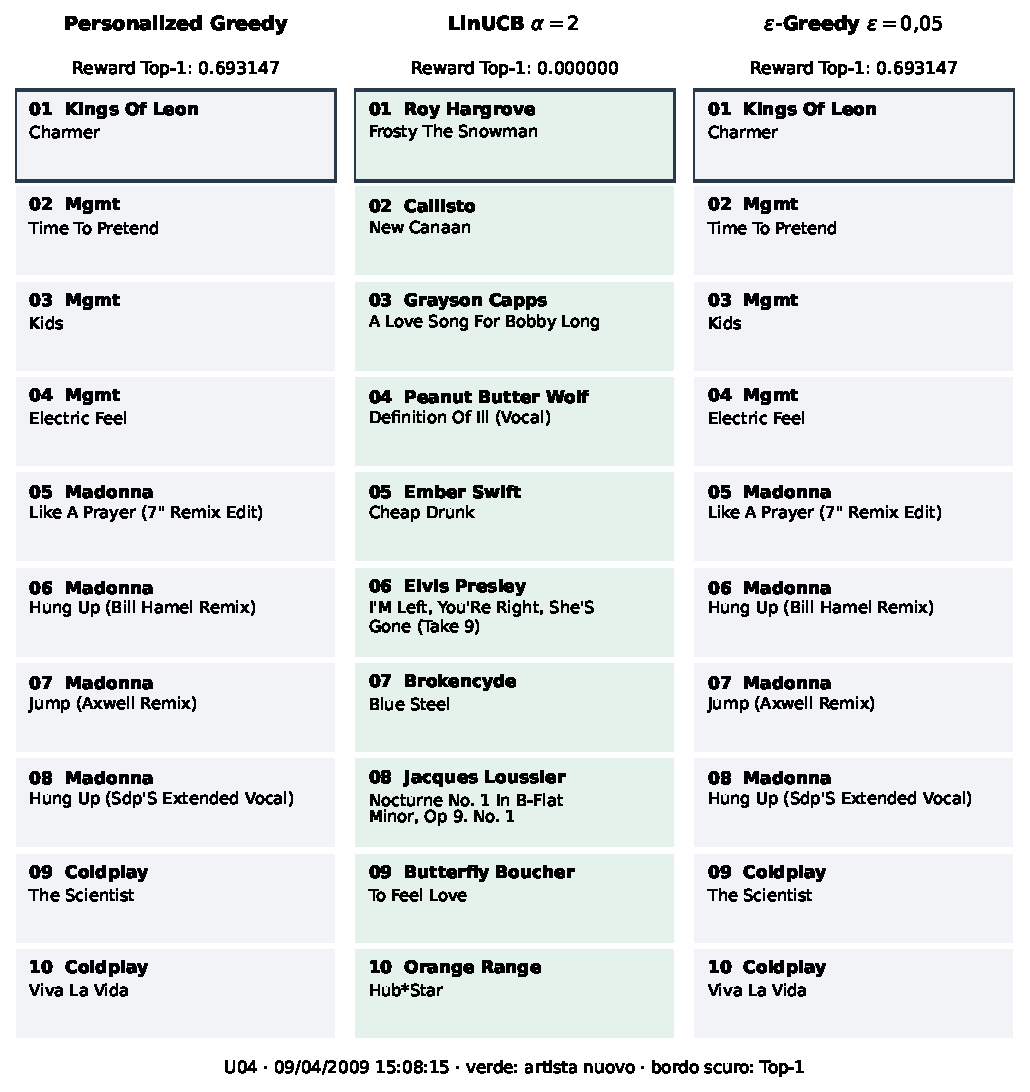
\includegraphics[width=\linewidth]{qualitative_U04.pdf}
\caption{Top-10 reali per U04, stesso utente e istante della Tabella~\ref{tab:u04}. Il verde contrassegna un artista mai ascoltato prima del decision point; il bordo scuro evidenzia la Top-1. Greedy ed $\varepsilon$-Greedy coincidono, mentre LinUCB cambia tutti gli artisti. Titoli, ordine, flag e reward sono letti dalla cache verificata, senza scansioni o nuove decisioni. Un artista nuovo non implica un successivo ascolto.}\label{fig:qualitative}
\end{figure}

\chapter{Incertezza e confronti appaiati}\label{ch:stat}
\section{Unità di ricampionamento e verifica delle metriche}
Le 82.905 decisioni non sono osservazioni indipendenti. Due sessioni dello stesso utente condividono preferenze, storia e spesso finestre future sovrapposte. Un bootstrap delle singole decisioni frammenterebbe artificialmente questa dipendenza e non riprodurrebbe la macro-aggregazione ufficiale. Il notebook statistico impiega perciò l'utente come unità di ricampionamento \cite{efron1993,field2007}. Il riferimento al bootstrap per cluster motiva tale scelta, senza garantire validità sotto qualsiasi dipendenza fra utenti.

Prima dell'inferenza, i checkpoint vengono allineati per utente e timestamp fra tutte le policy. Gli ascolti originali consentono di ricostruire il set di artisti rilevanti in $(t,t+7d]$; il ranking viene deduplicato con la prima occorrenza e IDCG segue l'Equazione~\ref{eq:ndcg}. Le medie utente ricostruite vengono confrontate agli aggregati per reward, NDCG, track novelty, artist novelty e ILD a @5, @10 e @20. Il notebook impone tolleranza assoluta $10^{-12}$ e relativa zero; la reward coincide anche a livello di decisione, con errore massimo registrato pari a zero.

Questa verifica è essenziale: una formula apparentemente simile potrebbe usare un diverso denominatore IDCG, trattare i duplicati come item distinti o pesare gli utenti in funzione delle loro sessioni. In tali casi gli intervalli descriverebbero una metrica diversa da quella selezionata in validation. La coverage globale non viene trasformata impropriamente in media individuale e non riceve gli intervalli seguenti.

L'inferenza completa quindi la verifica dell'obiettivo: la vicinanza delle medie non prova equivalenza dell'accuratezza, così come un incremento puntuale di novelty non ne descrive da solo l'incertezza fra utenti.

\section{Bootstrap appaiato}
Per ciascuna metrica si dispone del vettore delle 562 medie utente $\overline M^\pi_u$ della policy $\pi$. In ogni replica $b$ si estraggono con reinserimento 562 indici utente, usando gli stessi indici per tutte le policy:
\begin{align}
\widehat M_b^\pi&=\frac1{562}\sum_{j=1}^{562}\overline M^\pi_{u_j^{(b)}},\\
\widehat\delta_b^{\pi,\rho}
&=\frac1{562}\sum_{j=1}^{562}
\left(\overline M^\pi_{u_j^{(b)}}-\overline M^\rho_{u_j^{(b)}}\right).
\end{align}
Ogni media utente mantiene insieme tutta la sua sequenza temporale. Il notebook usa 10.000 replicazioni, seed 20261022 e quantili percentile 0,025 e 0,975. Non si sottraggono gli estremi di due intervalli marginali: la differenza è calcolata su coppie dello stesso utente, preservando la covariazione fra policy.

\begin{table}[htbp]\centering\small
\begin{tabular}{lrrr}
\toprule
Metrica & $\Delta$ & IC 95\% inf. & IC 95\% sup. \\
\midrule
average\_reward & -0,059984 & -0,091307 & -0,028959 \\
ndcg@10 & -0,001055 & -0,006601 & +0,004389 \\
track\_novelty@10 & +0,108348 & +0,096463 & +0,120665 \\
artist\_novelty@10 & +0,101535 & +0,086635 & +0,117116 \\
artist\_ild@10 & +0,079533 & +0,068874 & +0,090527 \\
\bottomrule
\end{tabular}

\caption{LinUCB $\alpha=2$ meno Personalized Greedy nel test: differenze appaiate e IC bootstrap al 95\% (percentile), dagli output verificati del notebook statistico.}\label{tab:ci}
\end{table}

\section{Interpretazione degli effetti}
Per NDCG@10 la differenza puntuale è $-0{,}001055$ e l'intervallo include zero. I dati e questo metodo non permettono di affermare una differenza direzionale affidabile fra LinUCB e Greedy. L'assenza di evidenza non è prova di equivalenza: questa richiederebbe margini di equivalenza motivati prima dell'analisi e una procedura dedicata. È corretto descrivere vicinanza numerica, dichiarandone l'incertezza.

Per Average Reward la differenza è $-0{,}059984$ e l'intervallo $[-0{,}091307;-0{,}028959]$ esclude zero. Il minor proxy medio di LinUCB è quindi più stabile rispetto alla variabilità fra utenti. Il risultato riguarda una differenza nella media di $\ln(1+n)$, non una perdita pari a 0,06 ascolti e neppure una percentuale causale di soddisfazione.

TN, AN e ILD presentano incrementi con intervalli interamente positivi. Gli effetti sono espressi nelle unità naturali delle metriche: per esempio $+0{,}108348$ di TN corrisponde a circa 10,83 punti percentuali, non al 10,83\% relativo. L'incremento di AN è particolarmente interpretabile perché Greedy ha AN@10 pari a zero.

\figura{paired_ci.pdf}{1}{Differenze appaiate LinUCB meno Greedy con IC bootstrap al 95\%. Le tre scale orizzontali separano reward, NDCG e composizione delle liste; lo zero tratteggiato è il riferimento di ciascun pannello. I valori esatti sono nella Tabella~\ref{tab:ci}, senza costruire un'utilità complessiva.}{fig:ci}

Rispetto a $\varepsilon$-Greedy, LinUCB ha $\Delta$ NDCG@10 $+0{,}008848$, IC bootstrap al 95\% $[0{,}003464;0{,}014129]$. La differenza di reward è $-0{,}016644$, IC bootstrap al 95\% $[-0{,}046835;0{,}013173]$, quindi non è chiaramente direzionale secondo questo intervallo. Anche in questo confronto novelty e ILD favoriscono numericamente LinUCB; non si usa l'inferenza per scegliere retroattivamente un nuovo modello.

\section{Limiti dell'inferenza}
L'analisi è post-hoc. Le metriche e i confronti sono correlati e gli intervalli sono nominali, senza correzioni per confronti multipli. Un intervallo che esclude zero non equivale a una garanzia simultanea su tutte le conclusioni. Le finestre temporali condivise fra utenti, le mode musicali e il modello LinUCB comune possono generare dipendenze fra cluster che il bootstrap per utente non rappresenta.

Si ricampionano le prestazioni di traiettorie già prodotte, senza riaddestrare la policy per ogni replica: l'incertezza è condizionata al protocollo, alla popolazione, al seed e all'esecuzione congelata. Non include tutta la variabilità da un nuovo training o da un nuovo scenario temporale. Un'analisi futura potrebbe considerare blocchi temporali comuni e repliche predefinite con più seed, ma tali esperimenti non sono stati eseguiti per questa relazione.

\chapter{Discussione e conclusioni}\label{ch:conclusioni}
\section{Risposta alla domanda di ricerca}
La domanda iniziale chiedeva se un modello contestuale con esplorazione potesse mantenere pertinenza aumentando novelty e diversità. Il test conferma anzitutto la necessità di una baseline forte: Greedy anticipa gli artisti futuri molto meglio di Random e Popularity. LinUCB raggiunge un NDCG@10 vicino, senza dimostrare superiorità sul riferimento personalizzato. Il passaggio dalla validation al test inverte il loro ordine numerico; il bootstrap appaiato non individua una direzione affidabile per questo piccolo scarto, né dimostra equivalenza.

Il vantaggio più netto di LinUCB riguarda la composizione delle liste. Rispetto a Greedy, propone più item mai ascoltati e più artisti nuovi, e riduce le ripetizioni dello stesso artista nella Top-10. Gli intervalli appaiati supportano la direzione di questi effetti nel campione analizzato. Il costo è una reward proxy media inferiore, con intervallo che esclude zero. La risposta alla domanda iniziale è quindi un compromesso documentato: vicinanza nell'accuratezza di ranking, maggiore apertura delle liste e minore allineamento Top-1 all'intensità degli ascolti futuri dell'artista.

L'incremento della novelty non identifica automaticamente la rilevanza dei nuovi contenuti. Un artista nuovo può non essere ascoltato nei sette giorni successivi; un artista noto può essere una proposta appropriata e desiderata. Gli esempi qualitativi rendono visibile questa asimmetria: liste diverse possono essere tutte familiari, mentre una lista ricca di artisti nuovi può avere reward nulla. Per un prodotto reale, il peso di questi aspetti richiederebbe obiettivi espliciti ed evidenze di utilizzo.

Il risultato è leggibile grazie al legame fra componenti e protocollo: stato cronologico e feedback differito definiscono l'informazione ammessa; pool comuni rendono confrontabili le opportunità; warm-up e scaler separano preparazione e valutazione; selezione in validation e congelamento preservano il ruolo del test. Macro-media e bootstrap per utente collegano infine le conclusioni all'unità di analisi scelta. Questi accorgimenti sostengono il confronto entro il protocollo adottato, senza dimostrare che ogni singola scelta architetturale sia ottimale.

\section{Limiti del protocollo e dell'architettura}
Il vincolo principale è l'assenza di esposizioni registrate. Non sono disponibili le azioni di una logging policy né le propensioni necessarie a IPS/SNIPS. A differenza di una valutazione offline su traffico randomizzato \cite{li2010offline}, l'esperimento non stima il reward controfattuale di una raccomandazione. L'ambiente assegna a ogni scelta un valore ricostruito dalla stessa sequenza di ascolti futura, che non cambia quando cambia la policy.

La reward artist-level valorizza il riascolto di qualunque traccia dell'artista selezionato. Una raccomandazione con titolo poco pertinente può così ottenere reward elevata; una buona scoperta ascoltata oltre sette giorni può ottenere zero. Il logaritmo attenua gli ascolti estremi, ma la misura rimane influenzata dall'attività e non corrisponde a soddisfazione dichiarata. La rilevanza binaria per NDCG considera invece solo la presenza dell'artista futuro: le due metriche valutano obiettivi connessi ma diversi.

L'eleggibilità seleziona utenti attivi in tutti i periodi e restringe la generalizzabilità ai profili persistenti. Il dataset, storico e composto da utenti Last.fm, non rappresenta necessariamente una piattaforma contemporanea o un ascoltatore occasionale. Gli ID mancanti e i fallback per nome preservano gli eventi, ma non risolvono sinonimie e omonimie: un nome non collegato al relativo MBID può restare un'entità distinta. La scelta di non unificare con statistiche future evita invece una riconciliazione retrospettiva nell'osservazione della policy.

La generazione lessicografica dei pool Personal e Discovery limita quali item entrano nell'azione. L'esplorazione non raggiunge contenuti non ancora osservati globalmente e il modello non usa caratteristiche audio o semantiche. Anche la ILD distingue soltanto identità artista: due artisti simili possono essere valutati come pienamente diversi. La coverage dipende dal candidato esposto, non da un catalogo universale.

Infine, il modello lineare condiviso assume che le feature bastino a spiegare una parte stabile dell'utilità. Le preferenze possono essere non lineari e variare nel tempo. Il sistema non include una procedura di forgetting o una prova di calibrazione dell'incertezza. I confronti non isolano ogni feature o il solo meccanismo esplorativo; la conclusione riguarda la pipeline implementata.

\figura{tradeoff.pdf}{.95}{Trade-off held-out fra NDCG@10, artist novelty e ILD. I punti sono aggregati macro per utente; le distanze nel grafico non costituiscono test di significatività.}{fig:tradeoff}

\section{Sviluppi futuri}
Un'estensione prioritaria sarebbe acquisire esposizioni, feedback espliciti e propensioni della logging policy, con un protocollo di raccolta che consenta valutazione controfattuale e sperimentazione online. Una prova controllata potrebbe misurare se nuove proposte producono ascolti successivi e come incidano sulla soddisfazione, senza inferirlo dal presente proxy.

Sul piano modellistico, feature musicali o embedding potrebbero rappresentare similarità oltre l'identità artista; un confronto predefinito con modelli di diversa capacità chiarirebbe il contributo della linearità. Un'ablation delle feature e dei pool, mantenendo gli stessi vincoli temporali, aiuterebbe a separare effetto del candidato, rappresentazione e bonus esplorativo. Una diversa generazione di candidati richiederebbe però un nuovo esperimento, senza reinterpretare i risultati congelati.

Sul piano statistico, più seed e periodi di test pianificati consentirebbero di studiare la stabilità temporale. L'ottimizzazione delle risorse dovrebbe continuare tramite riuso di artefatti immutabili e replay indipendenti, verificando equivalenza prima di nuove run. Il contributo del progetto è anche questa disciplina sperimentale: identità coerenti, causalità verificata, selezione antecedente al test e provenienza leggibile rendono i risultati discutibili e riproducibili.

\clearpage\addcontentsline{toc}{chapter}{Bibliografia}
\bibliographystyle{plain}
\bibliography{references}
\appendix
\chapter{Tracciabilità e griglia completa}\label{app:repro}
La relazione legge gli aggregati ufficiali senza rieseguire le policy. Lo script \path{report/build_assets.py} costruisce tabelle e grafici dai CSV, estrae figure EDA dagli output incorporati, verifica la cache qualitativa e conserva le tabelle statistiche già calcolate. Le fonti sono:
\begin{quote}\small
\path{experiments/results/validation/ea8616724509-5b076e7a/runs.csv}\\
\path{experiments/results/test/044f9269d4e3-5b076e7a/runs.csv}\\
\path{experiments/configs/final_selection_manifest.json}\\
\path{notebooks/03_statistical_analysis.ipynb}\\
\path{notebooks/data/qualitative_examples.json}
\end{quote}
Il dataset canonico ha SHA-256
\begin{quote}\small\path{5b076e7a1cb3646f58499d53976630528ecd9ac1a2431cb9f8c919a768c7a04a}.\end{quote}
Gli hash logici delle configurazioni sono
\begin{quote}\small
Validation: \path{ea8616724509edd297d13b5c83a38b14bb758d3148323a51fe123d997ec835f6}\\
Test: \path{044f9269d4e3820b8a2ff3e23bd6e191878ccfc421bc6532ac8f5d2ab15b983b}.
\end{quote}
La validation fa riferimento al commit \metric{f67c7d9}; il test al checkout \metric{4cd1fe0}, con preparazione del runner \metric{341f047}. Il manifesto conserva gli ID delle run selezionate prima del test. I digest completi degli input della relazione e gli ID delle 36+5 run sono in \metric{report/data/provenance.json}. Queste evidenze collegano le tabelle agli aggregati; non costituiscono una nuova verifica byte per byte dei molti gigabyte dei JSONL dettagliati.

La predefinizione dello scenario principale è verificabile nel commit del 7 ottobre 2026
\begin{quote}\small\path{c7167312f55fdacd86e4183bfd80a3d1b02d5b55}.\end{quote}
Il README del runner, righe 38--56 in quella revisione, fissa $N=100$ a priori, limita $N=50/200$ alla sensibilità e riserva la selezione a NDCG@10, poi reward e parametro minore. Configurazione e selettore della stessa revisione applicano quei vincoli. È documentazione antecedente ai risultati, non una preregistrazione formale.

Le configurazioni storiche mantengono il testo \metric{Dataset/...}, mentre la directory fisica è \metric{dataset}. Windows risolve la differenza di maiuscola; su filesystem case-sensitive si usa l'alias locale documentato. I dati delle run storiche e i loro hash non vengono rigenerati per adattarli al nome della directory.

I checkpoint persistenti verificano identità, seed e digest di ogni run. Il marker atomico segue il JSONL e ne conserva il checksum. La ripresa accetta solo run complete, ricostruisce istanze indipendenti e impedisce duplicazioni nell'aggregato.

\begin{table}[htbp]\centering\scriptsize
\begin{tabular}{lrrrrrr}
\toprule
Policy & $C_I@5$ & $C_G@5$ & $C_I@10$ & $C_G@10$ & $C_I@20$ & $C_G@20$ \\
\midrule
Random & 0,739289 & 0,866985 & 0,820794 & 0,925142 & 0,883490 & 0,960931 \\
Global Popularity & 0,001742 & 0,000298 & 0,003483 & 0,000298 & 0,008882 & 0,001193 \\
Personalized Greedy & 0,171543 & 0,192663 & 0,258447 & 0,284223 & 0,388889 & 0,418729 \\
$\varepsilon$-Greedy & 0,360850 & 0,454817 & 0,472309 & 0,575902 & 0,610763 & 0,710409 \\
LinUCB & 0,268722 & 0,331643 & 0,363636 & 0,447062 & 0,469697 & 0,572323 \\
\bottomrule
\end{tabular}

\caption{Coverage della validation principale per le configurazioni congelate, con cutoff espliciti.}
\end{table}

\clearpage\small
\begin{longtable}{rlrrr}
\caption{Griglia ufficiale di validation: 36 run.}\\
\toprule N & Policy & Parametro & NDCG@10 & Reward \\
\midrule\endfirsthead
\toprule N & Policy & Parametro & NDCG@10 & Reward \\
\midrule\endhead
50 & $\varepsilon$-Greedy & 0.05 & 0,258463 & 0,931208 \\
50 & $\varepsilon$-Greedy & 0.1 & 0,247923 & 0,885167 \\
50 & $\varepsilon$-Greedy & 0.2 & 0,227607 & 0,794801 \\
50 & Personalized Greedy & -- & 0,268507 & 0,975219 \\
50 & LinUCB & 0 & 0,256346 & 0,818279 \\
50 & LinUCB & 0.1 & 0,263883 & 0,936416 \\
50 & LinUCB & 0.25 & 0,263809 & 0,935975 \\
50 & LinUCB & 0.5 & 0,263789 & 0,934879 \\
50 & LinUCB & 1 & 0,263613 & 0,933102 \\
50 & LinUCB & 2 & 0,263452 & 0,928883 \\
50 & Global Popularity & -- & 0,052096 & 0,308597 \\
50 & Random & -- & 0,065606 & 0,095330 \\
100 & $\varepsilon$-Greedy & 0.05 & 0,265987 & 1,012495 \\
100 & $\varepsilon$-Greedy & 0.1 & 0,254587 & 0,960985 \\
100 & $\varepsilon$-Greedy & 0.2 & 0,234917 & 0,870854 \\
100 & Personalized Greedy & -- & 0,276427 & 1,060560 \\
100 & LinUCB & 0 & 0,270426 & 0,882643 \\
100 & LinUCB & 0.1 & 0,284684 & 1,004397 \\
100 & LinUCB & 0.25 & 0,284530 & 1,003799 \\
100 & LinUCB & 0.5 & 0,284789 & 1,003569 \\
100 & LinUCB & 1 & 0,285205 & 1,004232 \\
100 & LinUCB & 2 & 0,285640 & 1,003704 \\
100 & Global Popularity & -- & 0,041145 & 0,308597 \\
100 & Random & -- & 0,066118 & 0,097295 \\
200 & $\varepsilon$-Greedy & 0.05 & 0,262647 & 1,081188 \\
200 & $\varepsilon$-Greedy & 0.1 & 0,252239 & 1,027739 \\
200 & $\varepsilon$-Greedy & 0.2 & 0,230979 & 0,919576 \\
200 & Personalized Greedy & -- & 0,273409 & 1,132060 \\
200 & LinUCB & 0 & 0,271897 & 0,949816 \\
200 & LinUCB & 0.1 & 0,293634 & 1,101288 \\
200 & LinUCB & 0.25 & 0,293681 & 1,100327 \\
200 & LinUCB & 0.5 & 0,293727 & 1,099923 \\
200 & LinUCB & 1 & 0,293811 & 1,099431 \\
200 & LinUCB & 2 & 0,293715 & 1,097895 \\
200 & Global Popularity & -- & 0,041145 & 0,308597 \\
200 & Random & -- & 0,063062 & 0,091953 \\
\bottomrule\end{longtable}
\normalsize

\end{document}
